\section{Property\-File Class Reference}
\label{classPropertyFile}\index{PropertyFile@{PropertyFile}}
This is the implementation of the key\-Value\-Store on filesystem.  


{\tt \#include $<$Property\-File.h$>$}

Inheritance diagram for Property\-File:\begin{figure}[H]
\begin{center}
\leavevmode
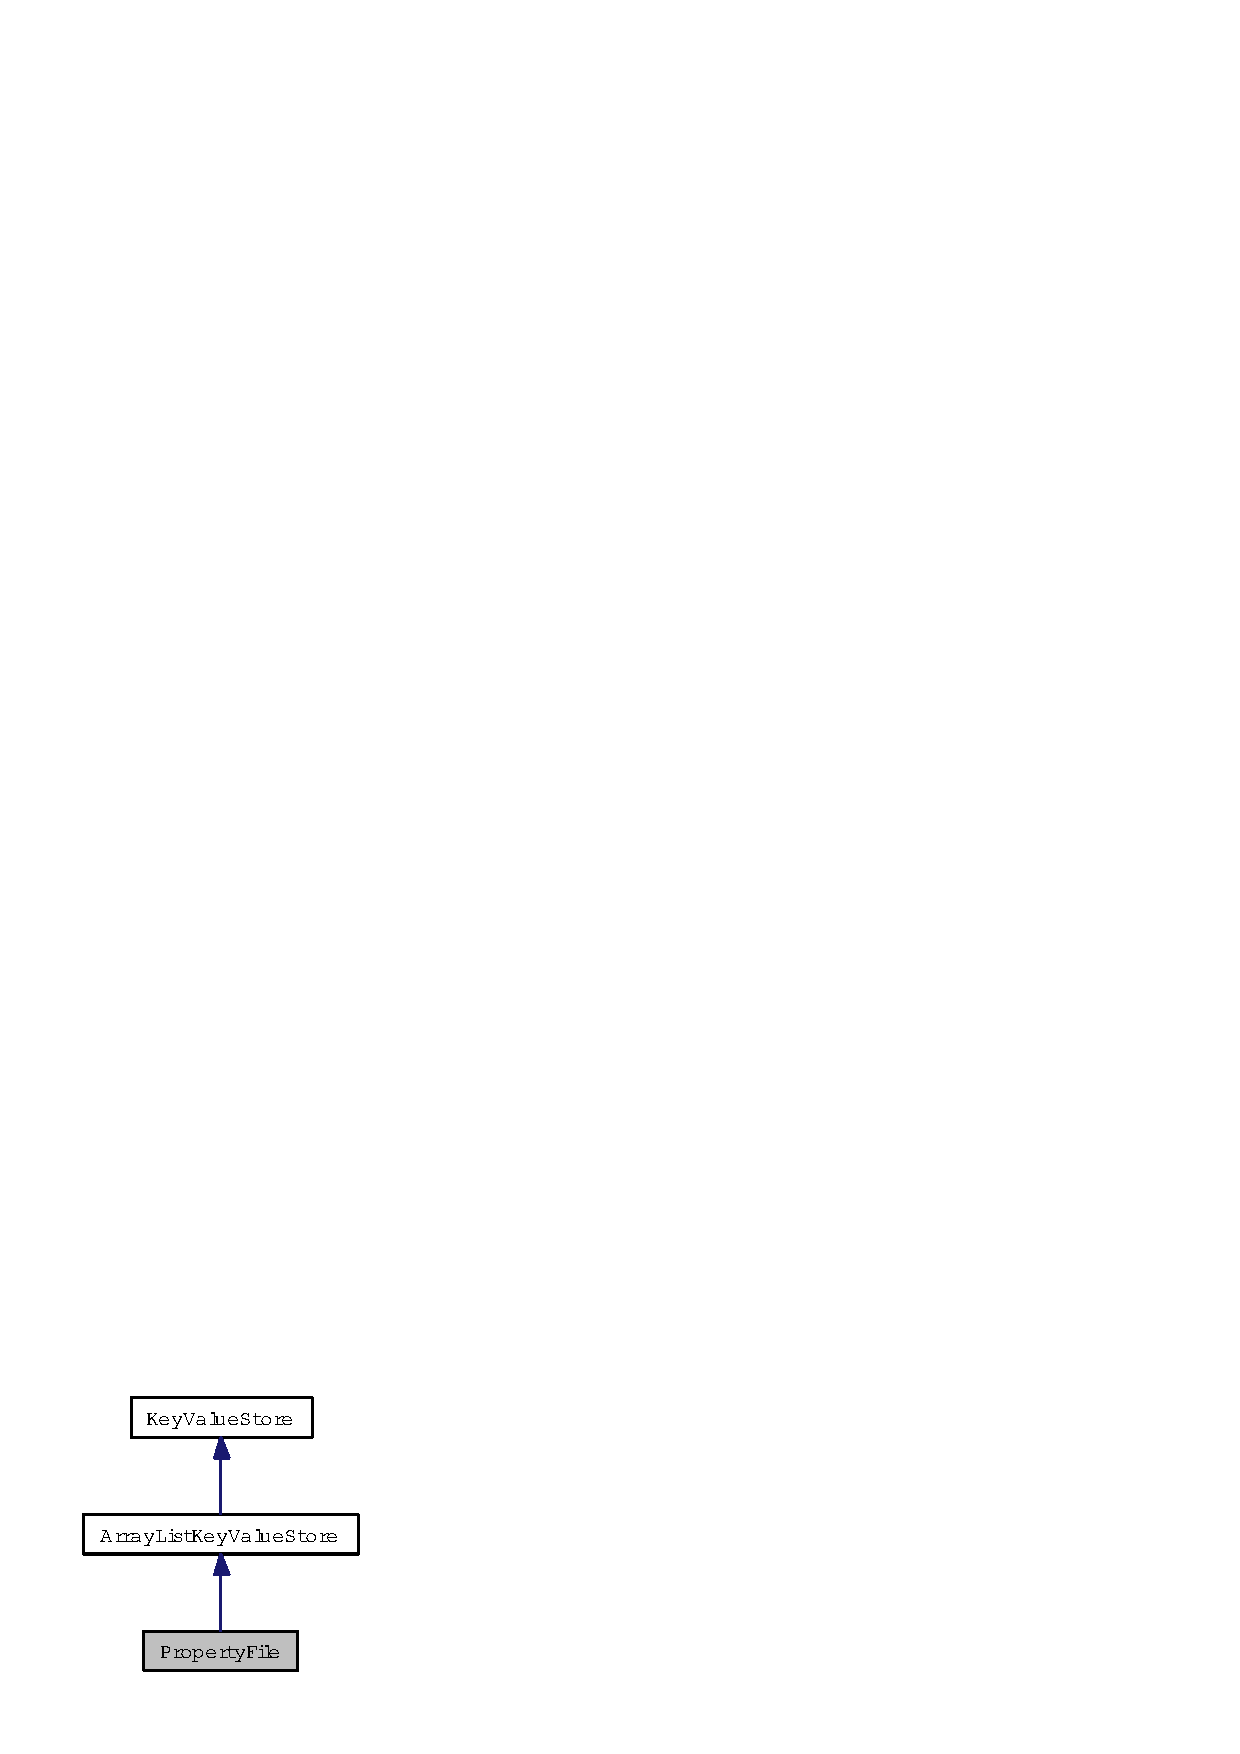
\includegraphics[width=88pt]{classPropertyFile__inherit__graph}
\end{center}
\end{figure}
Collaboration diagram for Property\-File:\begin{figure}[H]
\begin{center}
\leavevmode
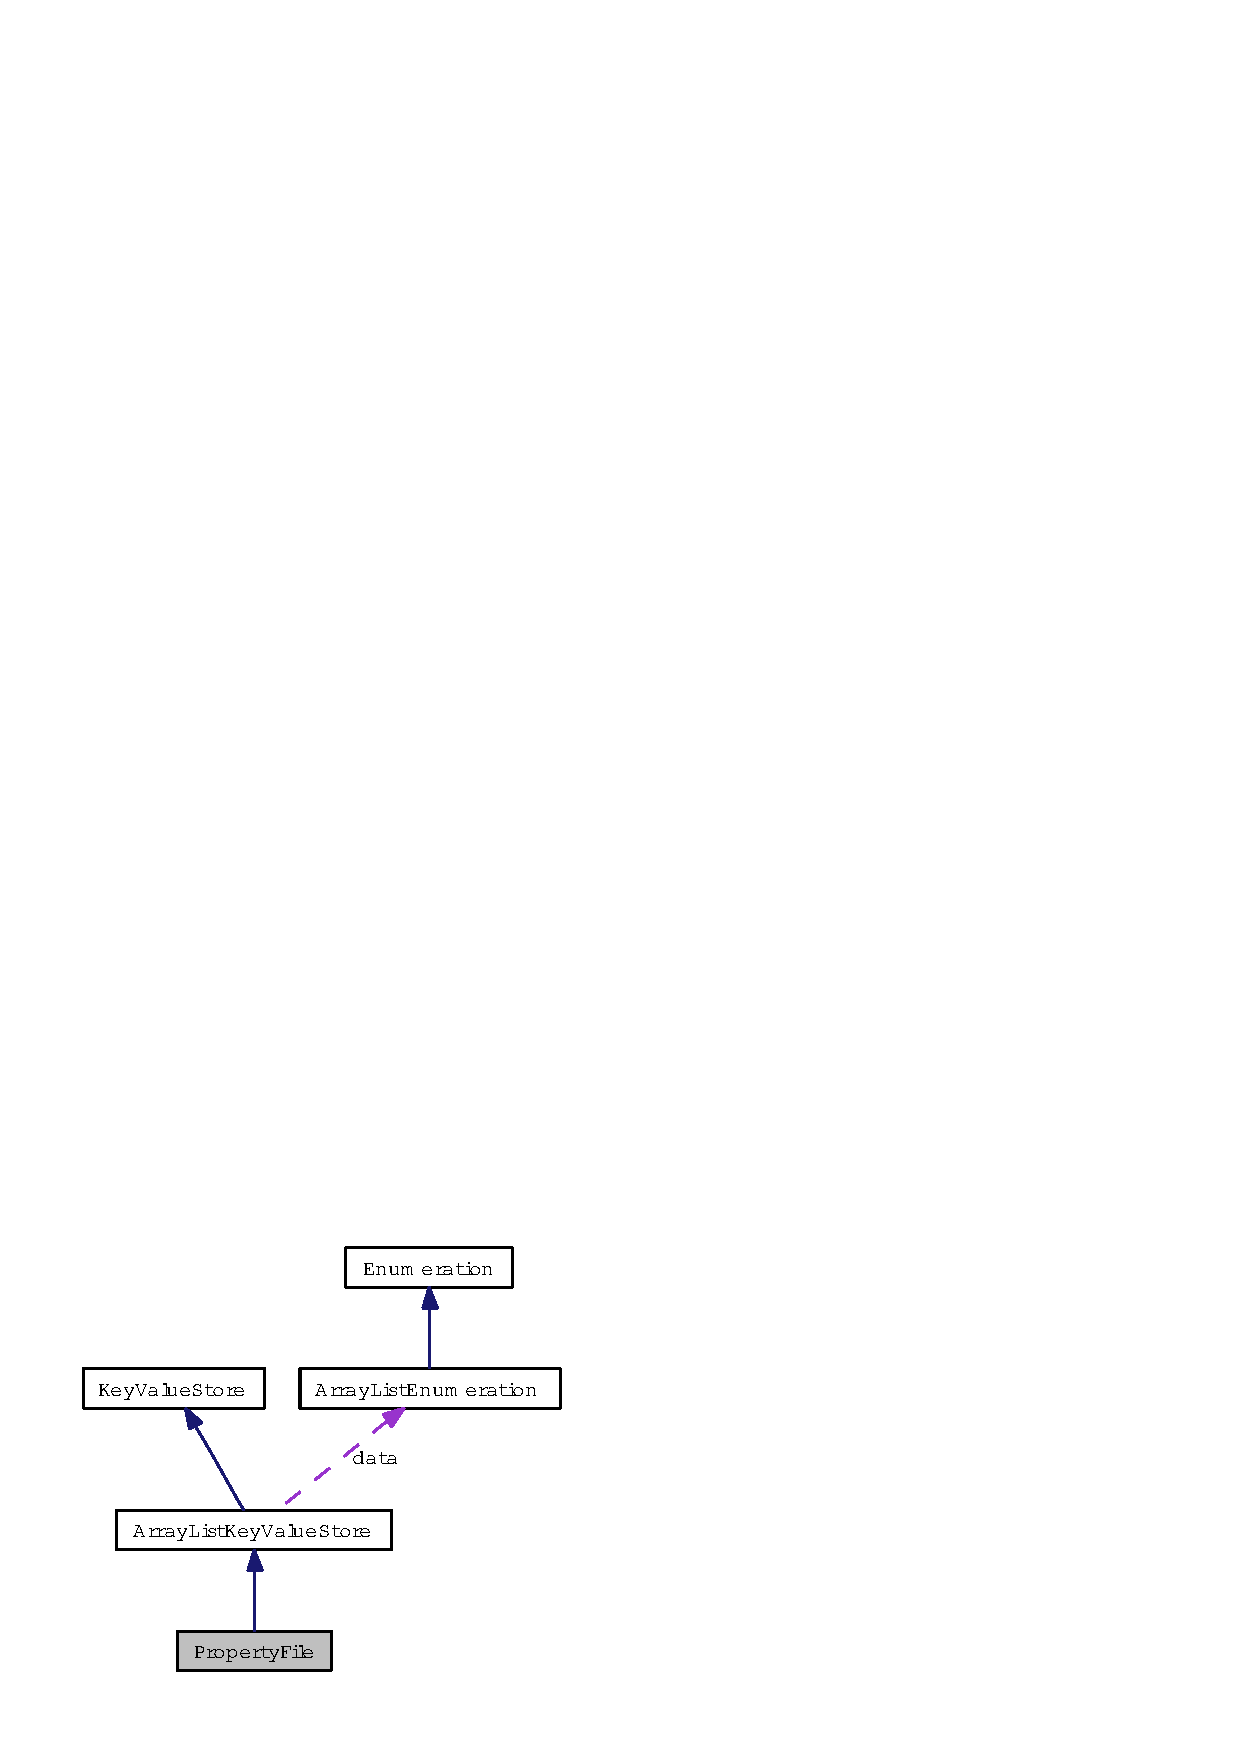
\includegraphics[width=136pt]{classPropertyFile__coll__graph}
\end{center}
\end{figure}
\subsection*{Public Member Functions}
\begin{CompactItemize}
\item 
{\bf Property\-File} (const char $\ast$n)\label{classPropertyFile_90f1d7a2899f43ced063e4aed9d5a7f0}

\begin{CompactList}\small\item\em The name of the general node. \item\end{CompactList}\item 
int {\bf save} ()\label{classPropertyFile_f6258c0d8d6360f4a024384617d4009e}

\begin{CompactList}\small\item\em Save the current properties that are in the data arraylist in the filesystem. \item\end{CompactList}\end{CompactItemize}


\subsection{Detailed Description}
This is the implementation of the key\-Value\-Store on filesystem. 

It provides methods to read and write in the filesystem the arraylist of Key\-Value\-Pair 



The documentation for this class was generated from the following file:\begin{CompactItemize}
\item 
src/include/common/base/util/Property\-File.h\end{CompactItemize}
